\documentclass[a4paper,10pt]{article}
\usepackage{graphicx}
%opening
\title{Software defined radio for MyriaNed}
\author{Fasika A.Assegei}
\begin{document}
\maketitle
\newpage
\begin{abstract}
GNU Radio is an open source software-defined radio project, and the
USBM is hardware designed specifically for use with GNU Radio, made
by Mediatronix. Together, these two pieces have been used to
implement a low cost, software-defined radios. In this thesis, we
discuss the design of a software-defined radio application for
wireless sensor networks, built using the open source GNU Radio and
a proprietary hardware made by Mediatronix.
\newline
In the second part of the thesis, the time synchronization of the
wireless sensor nodes will be dealt with. An algorithm developed for
a distributed multihop sensor network is presented with the results
of the simulation conducted.
\end{abstract}
\newpage
\tableofcontents
\newpage
\section{Introduction}
\newpage
\section{Software Defined Radio}
A cognitive radio is a........ A software-defined radio (SDR) is a
radio communication system that performs radio signal modulation and
demodulation in software.The exact extent to which a particular
radio system may be considered an SDR is not entirely clear because
the SDR community has not yet formulated definitive answers to
questions regarding the types of processor upon which the software
can run, or the percentage of total signal processing that must be
performed in software. However, it is clear that the philosophy
behind the SDR concept is that the software should operate as close
to the antenna as possible (in terms of intervening signal
processing stages), and this software should run on a general
purpose computer. See Figure $\ref{fig:blockdiagram}$ for the block
diagram of an ideal SDR.
\begin{figure}
\centering
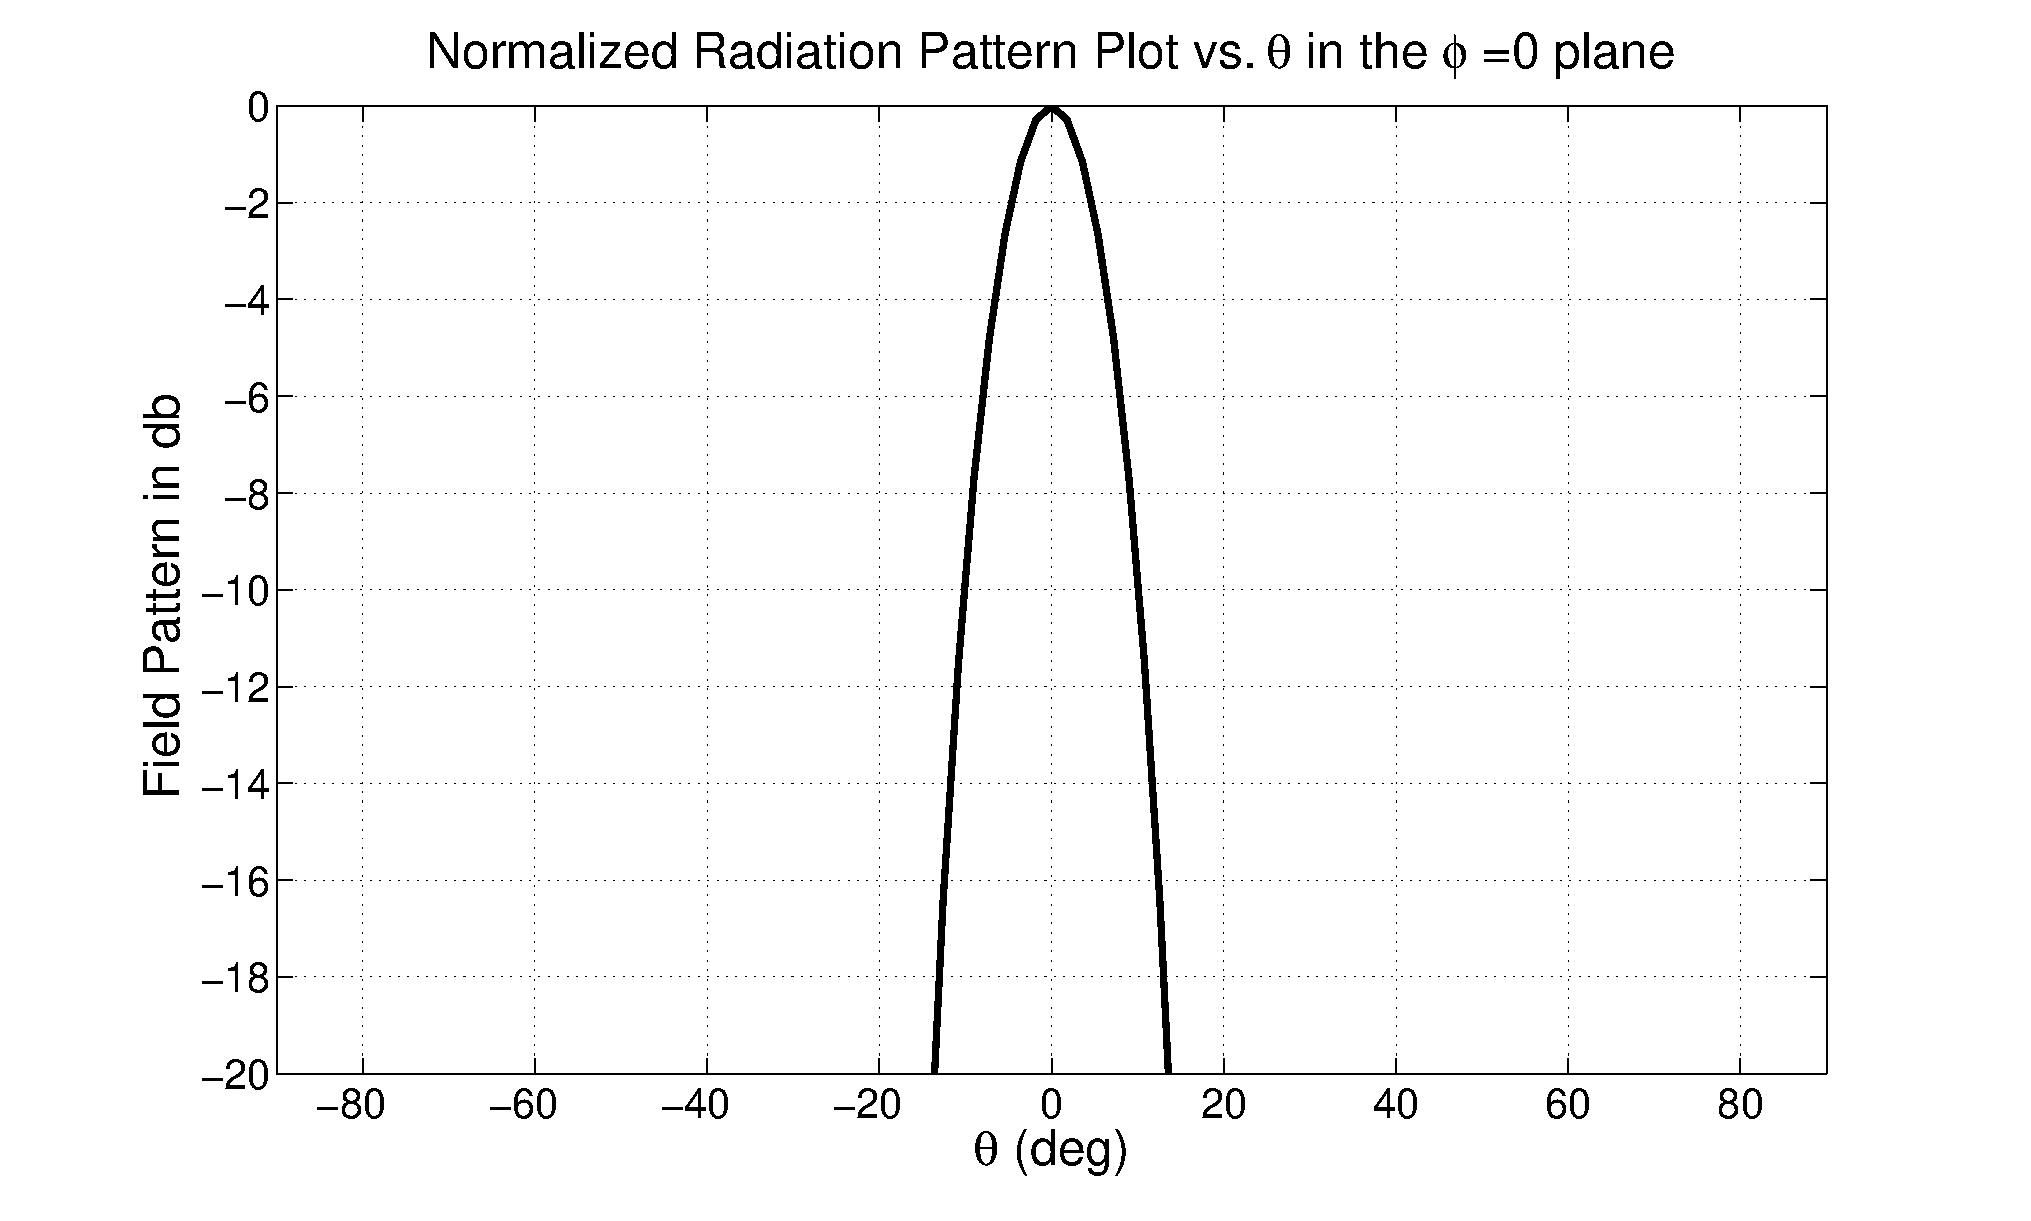
\includegraphics[width=0.5 \textwidth]{Broadside}
\caption{Block Diagram of an SDR} \label{fig:blockdiagram}
\end{figure}
The impetus of SDR research is a desire to shift the radio
engineering problem from the hardware domain to the software domain.
The advantage of this problem-space translation is that the software
domain provides an inherently more flexible, predictable,
repeatable, and accessible solution space than does the hardware
domain. In the software domain, all radios are differentiated solely
by the software required to implement them. Therefore, a single SDR
system could become one of any number of RF transceivers (e.g., GPS,
802.11, HDTV) by simply executing a different block of code residing
in memory. Of course, realizing the ideal SDR of Figure means
overcoming some formidable obstacles. Consider the components of
this system: \newline 1. Ideal transmit and receive antennas - These
antennas can operate at the carrier frequencies of all radio signals
of interest. \newline 2. Ideal analog-to-digital and
digital-to-analog converters - These devices have sampling rates
greater than two times the carrier frequency of all radio signals of
interest. At this sampling rate, all signals of interest can be
processed at their carrier frequency.\newline 3. Ideal computer -
This computer has sufficient processing power to handle the realtime
signal processing and protocol management demands for all radio
signals of interest. In reality, antennas must be designed for
operation within a particular frequency band, modern
analog-to-digital converters (ADCs) and digital-to-analog converters
(DACs) are not fast enough to process a large portion of the
occupied spectrum, and current general purpose computers are still
not sufficient to handle the real-time demands of many applications.
\newpage
\section{GNU Radio and RF frontend}
\subsection{GNU Radio}
The GNU Radio project is a framework for performing digital signal
processing and controlling software defined radio. It allows for
rapid development of signal processing application by joining blocks
together to form a pipeline, taking the signal from reception to
useful output. A block is a small step of processing within a
pipeline, they range from file sources and sinks, to demodulators
and from packet parsers to PAL television decoders. Most blocks are
written in C++ with a frontend in python, the scripts that link the
pipeline stages are written in python. It is a future goal of the
project to allow entire applications to be written in C++, this well
reduce the overheads and allow some of the slower pipelines to run
in real time.
\subsection{RF Frontend}
\subsubsection{Introduction}
The RF front end that we use in this project is designed to be used
with the GNU radio software to receive and analyze the signals
received by the antenna. The device consists of a main board with
digital signal processors on it, along with connected daughter a
board which are specific to various frequency bands. The daughter
board is aimed at the 2.4GHz to 2.5GHz industrial, scientific and
medical band. This is the frequency band that wireless sensor nodes
use. The device is used to receive the signals from the wireless
sensor nodes so there is no transmitting feature on the device.
Together it can be set-up as a test facility, which can be used for
protocol-analysis, performance and quality measurements, and
actively participate in the communication with the wireless sensor
network.
\subsubsection{Block Diagram}
The block digram of the RF front end is shown below.
\subsubsection{Packet format}
The sensor nodes are equipped with the nordic transceiver nRF24LU1.
All communications are packet based and packets are sent at a rate
of 1Mb/s. Data is modulated using GFSK modulation, where a frequency
shift of +115KHz represents a binary 1, and -115KHz represents a
binary 0. The packet format is described below. \newline Packets are
made up of three sections, preamble, address and payload. The packet
is accompanied by a CRC at the end. All packets have a preamble to
inform other devices the start of the packet transmission.The
address part of the packet identifies the sender of the packet and
the data stored in the payload is formatted accordingly. The packet
is 313 bits long. The packet format is shown below. ( Figure). A
preamble is an 8 bit sequence of ones and zeros. It can be 01010101
if the address field starts with 0 and 10101010 if the address field
starts with 0. The address field is a 3 Byte field which describes
the address of the transmitting node. The Packet Identification
Device ( PID ) contains the length of the payload. In our case, the
payload is a 32 byte data. so, the filed remains constant for the
packets. The payload, as said earlier, is a
 32 byte followed by a 2 byte crc field.
\subsection{Detection of the signal}
The signal is first detected by the hardware front end within the
range of ISM band. The frequency that it is transmitted is fixed so
the receiver is also set to work with that frequency.The data is
modulated using Gaussian Frequency Shift Keying (GFSK) which is a
variant of Gaussian Minimum Shift Keying (GMSK) that has a specific
frequency shift of 115KHz. It has a symbol rate of 1MS/s, which,
when taken with the sampling rate of the GNU Radio in the 2.4GHz
band, give a total of four samples per symbol (bit). When these
parameters are passed to the GMSK demodulator from the GNU Radio
project it is able to demodulate the USBM packets. The signal is
then detected when the first 8 bits of the signal matches the
preamble.
\subsection{Deciphering the Packet}
Figure shows the stages that the signal received by the radio must
pass through in order to be processed. These modules are part of the
GNU Radio framework, from the USBM hardware, to the software filters
and demodulators that come with the software framework. The USBM
module was adapted in order to process the binary data that comes
from the demodulator. Figure 5.2: Flow of data within the GNU Radio
software. The hardware control, filters and GFSK demodulator are
part of the GNU Radio framework, however the USBM specific block was
written for deciphering the packets depending on a module previously
written by Dominic . The module works through a stream of data to
find the preamble and the crc of the packet at the correct distance
apart. It then takes the portion that represents the address and the
payload. Then, it creates a CRC using the crc16 CCITT algorithm. It
then compares the crc received and the crc calculated. If they
match, it returns the payload and the address of the packet. If they
dont match, it discards the packet and continues to search for the
other packet. The following figure shows the process of extracting
the payload from the data packet received from the GFSK demodulator.
\section{Conclusion and Recommendation}
\newpage
\begin{thebibliography}{}
\bibitem{1} R. Mirollo and S. Strogatz, Synchronization of pulse-coupled biological oscillators, SIAM J. Appl. Math, vol. 50, no. 6, pp. 1645-1662,Dec 1990.
\bibitem{2} Romer,K. Time Synchronization in Ad Hoc Networks. In: Proceedings of the Second ACM International Symposium on Mobile Ad Hoc Networking and Computing, Long Beach, California. 2001
\bibitem{3}
\bibitem{4}
\bibitem{5}
\bibitem{6}
\bibitem{7}
\bibitem{8}
\bibitem{9}
\bibitem{10}
\bibitem{11}
\bibitem{12}
\end{thebibliography}
\end{document}
